\documentclass[]{article}
\usepackage{lmodern}
\usepackage{amssymb,amsmath}
\usepackage{ifxetex,ifluatex}
\usepackage{fixltx2e} % provides \textsubscript
\ifnum 0\ifxetex 1\fi\ifluatex 1\fi=0 % if pdftex
  \usepackage[T1]{fontenc}
  \usepackage[utf8]{inputenc}
\else % if luatex or xelatex
  \ifxetex
    \usepackage{mathspec}
  \else
    \usepackage{fontspec}
  \fi
  \defaultfontfeatures{Ligatures=TeX,Scale=MatchLowercase}
\fi
% use upquote if available, for straight quotes in verbatim environments
\IfFileExists{upquote.sty}{\usepackage{upquote}}{}
% use microtype if available
\IfFileExists{microtype.sty}{%
\usepackage{microtype}
\UseMicrotypeSet[protrusion]{basicmath} % disable protrusion for tt fonts
}{}
\usepackage[margin=1in]{geometry}
\usepackage{hyperref}
\hypersetup{unicode=true,
            pdfborder={0 0 0},
            breaklinks=true}
\urlstyle{same}  % don't use monospace font for urls
\usepackage{color}
\usepackage{fancyvrb}
\newcommand{\VerbBar}{|}
\newcommand{\VERB}{\Verb[commandchars=\\\{\}]}
\DefineVerbatimEnvironment{Highlighting}{Verbatim}{commandchars=\\\{\}}
% Add ',fontsize=\small' for more characters per line
\usepackage{framed}
\definecolor{shadecolor}{RGB}{248,248,248}
\newenvironment{Shaded}{\begin{snugshade}}{\end{snugshade}}
\newcommand{\KeywordTok}[1]{\textcolor[rgb]{0.13,0.29,0.53}{\textbf{#1}}}
\newcommand{\DataTypeTok}[1]{\textcolor[rgb]{0.13,0.29,0.53}{#1}}
\newcommand{\DecValTok}[1]{\textcolor[rgb]{0.00,0.00,0.81}{#1}}
\newcommand{\BaseNTok}[1]{\textcolor[rgb]{0.00,0.00,0.81}{#1}}
\newcommand{\FloatTok}[1]{\textcolor[rgb]{0.00,0.00,0.81}{#1}}
\newcommand{\ConstantTok}[1]{\textcolor[rgb]{0.00,0.00,0.00}{#1}}
\newcommand{\CharTok}[1]{\textcolor[rgb]{0.31,0.60,0.02}{#1}}
\newcommand{\SpecialCharTok}[1]{\textcolor[rgb]{0.00,0.00,0.00}{#1}}
\newcommand{\StringTok}[1]{\textcolor[rgb]{0.31,0.60,0.02}{#1}}
\newcommand{\VerbatimStringTok}[1]{\textcolor[rgb]{0.31,0.60,0.02}{#1}}
\newcommand{\SpecialStringTok}[1]{\textcolor[rgb]{0.31,0.60,0.02}{#1}}
\newcommand{\ImportTok}[1]{#1}
\newcommand{\CommentTok}[1]{\textcolor[rgb]{0.56,0.35,0.01}{\textit{#1}}}
\newcommand{\DocumentationTok}[1]{\textcolor[rgb]{0.56,0.35,0.01}{\textbf{\textit{#1}}}}
\newcommand{\AnnotationTok}[1]{\textcolor[rgb]{0.56,0.35,0.01}{\textbf{\textit{#1}}}}
\newcommand{\CommentVarTok}[1]{\textcolor[rgb]{0.56,0.35,0.01}{\textbf{\textit{#1}}}}
\newcommand{\OtherTok}[1]{\textcolor[rgb]{0.56,0.35,0.01}{#1}}
\newcommand{\FunctionTok}[1]{\textcolor[rgb]{0.00,0.00,0.00}{#1}}
\newcommand{\VariableTok}[1]{\textcolor[rgb]{0.00,0.00,0.00}{#1}}
\newcommand{\ControlFlowTok}[1]{\textcolor[rgb]{0.13,0.29,0.53}{\textbf{#1}}}
\newcommand{\OperatorTok}[1]{\textcolor[rgb]{0.81,0.36,0.00}{\textbf{#1}}}
\newcommand{\BuiltInTok}[1]{#1}
\newcommand{\ExtensionTok}[1]{#1}
\newcommand{\PreprocessorTok}[1]{\textcolor[rgb]{0.56,0.35,0.01}{\textit{#1}}}
\newcommand{\AttributeTok}[1]{\textcolor[rgb]{0.77,0.63,0.00}{#1}}
\newcommand{\RegionMarkerTok}[1]{#1}
\newcommand{\InformationTok}[1]{\textcolor[rgb]{0.56,0.35,0.01}{\textbf{\textit{#1}}}}
\newcommand{\WarningTok}[1]{\textcolor[rgb]{0.56,0.35,0.01}{\textbf{\textit{#1}}}}
\newcommand{\AlertTok}[1]{\textcolor[rgb]{0.94,0.16,0.16}{#1}}
\newcommand{\ErrorTok}[1]{\textcolor[rgb]{0.64,0.00,0.00}{\textbf{#1}}}
\newcommand{\NormalTok}[1]{#1}
\usepackage{longtable,booktabs}
\usepackage{graphicx,grffile}
\makeatletter
\def\maxwidth{\ifdim\Gin@nat@width>\linewidth\linewidth\else\Gin@nat@width\fi}
\def\maxheight{\ifdim\Gin@nat@height>\textheight\textheight\else\Gin@nat@height\fi}
\makeatother
% Scale images if necessary, so that they will not overflow the page
% margins by default, and it is still possible to overwrite the defaults
% using explicit options in \includegraphics[width, height, ...]{}
\setkeys{Gin}{width=\maxwidth,height=\maxheight,keepaspectratio}
\IfFileExists{parskip.sty}{%
\usepackage{parskip}
}{% else
\setlength{\parindent}{0pt}
\setlength{\parskip}{6pt plus 2pt minus 1pt}
}
\setlength{\emergencystretch}{3em}  % prevent overfull lines
\providecommand{\tightlist}{%
  \setlength{\itemsep}{0pt}\setlength{\parskip}{0pt}}
\setcounter{secnumdepth}{0}
% Redefines (sub)paragraphs to behave more like sections
\ifx\paragraph\undefined\else
\let\oldparagraph\paragraph
\renewcommand{\paragraph}[1]{\oldparagraph{#1}\mbox{}}
\fi
\ifx\subparagraph\undefined\else
\let\oldsubparagraph\subparagraph
\renewcommand{\subparagraph}[1]{\oldsubparagraph{#1}\mbox{}}
\fi

%%% Use protect on footnotes to avoid problems with footnotes in titles
\let\rmarkdownfootnote\footnote%
\def\footnote{\protect\rmarkdownfootnote}

%%% Change title format to be more compact
\usepackage{titling}

% Create subtitle command for use in maketitle
\newcommand{\subtitle}[1]{
  \posttitle{
    \begin{center}\large#1\end{center}
    }
}

\setlength{\droptitle}{-2em}

  \title{}
    \pretitle{\vspace{\droptitle}}
  \posttitle{}
    \author{}
    \preauthor{}\postauthor{}
    \date{}
    \predate{}\postdate{}
  

\begin{document}

\section{Exercise 2: From Models to
Forecasts}\label{exercise-2-from-models-to-forecasts}

Note: This activity supplements material in Ecological Forecasting
Chapter 2 ``From Models to Forecasts'' As a class activity, please turn
in answers in Rmd format.

\subsection{Simulating the discrete-time
logistic}\label{simulating-the-discrete-time-logistic}

Define parameters

\begin{Shaded}
\begin{Highlighting}[]
\NormalTok{devtools}\OperatorTok{::}\KeywordTok{install_github}\NormalTok{(}\StringTok{"EcoForecast/ecoforecastR"}\NormalTok{)}
\end{Highlighting}
\end{Shaded}

\begin{verbatim}
## Skipping install of 'ecoforecastR' from a github remote, the SHA1 (2aca8d36) has not changed since last install.
##   Use `force = TRUE` to force installation
\end{verbatim}

\begin{Shaded}
\begin{Highlighting}[]
\NormalTok{r =}\StringTok{ }\DecValTok{1}\NormalTok{         ## intrinsic growth rate}
\NormalTok{K =}\StringTok{ }\DecValTok{10}\NormalTok{        ## carrying capacity      }
\NormalTok{n0 =}\StringTok{ }\NormalTok{.}\DecValTok{1}\NormalTok{       ## initial population size}
\NormalTok{NT =}\StringTok{ }\DecValTok{30}\NormalTok{       ## number of time steps to simulate}
\NormalTok{time =}\StringTok{ }\DecValTok{1}\OperatorTok{:}\NormalTok{NT}
\end{Highlighting}
\end{Shaded}

Iterative simulation

\begin{Shaded}
\begin{Highlighting}[]
\NormalTok{n =}\StringTok{ }\KeywordTok{rep}\NormalTok{(n0,NT)    ## vector to store results}
\ControlFlowTok{for}\NormalTok{(t }\ControlFlowTok{in} \DecValTok{2}\OperatorTok{:}\NormalTok{NT)\{}
\NormalTok{  n[t] =}\StringTok{ }\NormalTok{n[t}\OperatorTok{-}\DecValTok{1}\NormalTok{] }\OperatorTok{+}\StringTok{ }\NormalTok{r}\OperatorTok{*}\NormalTok{n[t}\OperatorTok{-}\DecValTok{1}\NormalTok{]}\OperatorTok{*}\NormalTok{(}\DecValTok{1}\OperatorTok{-}\NormalTok{n[t}\OperatorTok{-}\DecValTok{1}\NormalTok{]}\OperatorTok{/}\NormalTok{K)}
\NormalTok{\}}
\end{Highlighting}
\end{Shaded}

Plot results

\begin{Shaded}
\begin{Highlighting}[]
\KeywordTok{plot}\NormalTok{(time,n,}\DataTypeTok{ylim=}\KeywordTok{c}\NormalTok{(}\DecValTok{0}\NormalTok{,}\DecValTok{12}\NormalTok{),}\DataTypeTok{lwd=}\DecValTok{3}\NormalTok{,}\DataTypeTok{type=}\StringTok{'l'}\NormalTok{,}
     \DataTypeTok{bty=}\StringTok{'l'}\NormalTok{,}\DataTypeTok{cex.lab=}\FloatTok{1.5}\NormalTok{,}
     \DataTypeTok{xlab=}\StringTok{"Time"}\NormalTok{,}\DataTypeTok{ylab=}\StringTok{"Population Size"}\NormalTok{)}
\end{Highlighting}
\end{Shaded}

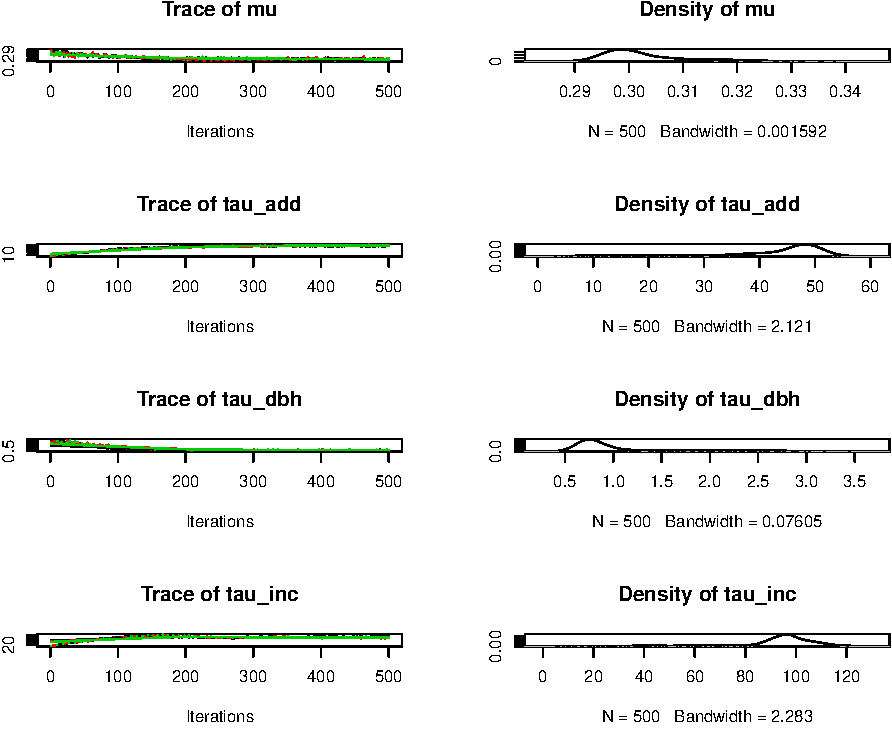
\includegraphics{Exercise_02_Logistic_files/figure-latex/unnamed-chunk-3-1.pdf}

\subsubsection{Problems}\label{problems}

\begin{enumerate}
\def\labelenumi{\arabic{enumi}.}
\tightlist
\item
  Generate plots of the logistic growth model at r = 1.95, 2.05, 2.5,
  and 2.8 Describe the trajectory observed in each case.
\end{enumerate}

\subsection{Probability distributions in
R}\label{probability-distributions-in-r}

Because it is a statistical language, there are a large number of
probability distributions in R by default and an even larger number that
can be loaded from packages. The table below gives a listing of the most
common distributions in R, the name of the function within R, and the
parameters of the distribution.

\begin{longtable}[]{@{}lll@{}}
\toprule
Distribution & R name & Parameters\tabularnewline
\midrule
\endhead
beta & beta & shape1, shape2, ncp\tabularnewline
Binomial & binom & size, prob\tabularnewline
Cauchy & cauchy & location, scale\tabularnewline
chi-squared & chisq & df, ncp\tabularnewline
exponential & exp & rate\tabularnewline
F & f & df1, df2, ncp\tabularnewline
gamma & gamma & shape, scale\tabularnewline
geometric & geom & prob\tabularnewline
hypergeometric & hyper & m, n, k\tabularnewline
log-normal & lnorm & meanlog, sdlog\tabularnewline
logistic & logis & location, scale\tabularnewline
Negative binomial & nbinom & size, prob\tabularnewline
Normal & norm & mean, sd\tabularnewline
Poisson & pois & lambda\tabularnewline
Student's t & t & df, ncp\tabularnewline
uniform & unif & min, max\tabularnewline
Weibull & weibull & shape, scale\tabularnewline
Wilcoxon & wilcox & m, n\tabularnewline
\bottomrule
\end{longtable}

There is a good chart at
\url{http://www.johndcook.com/distribution_chart.html} that describes
the relationships among the common distributions, and the Wikipedia
articles for most of them are good for quick reference.

R actually provides four related functions for each probability
distribution. These functions are called by adding a letter at the
beginning of the function name. The variants of each probability
distribution are:

\begin{itemize}
\tightlist
\item
  ``d'' = density: probability density function (PDF)
\item
  ``p'' = cumulative distribution function (CDF)
\item
  ``q'' = quantile: calculates the value associated with a specified
  tail probability, inverse of ``p''
\item
  ``r'' = random: simulates random numbers
\end{itemize}

The first argument to these functions is the same regardless of the
distribution and is x for ``d'', q for ``p'', p for ``q''and n for ``r''

All of this will make more sense once we consider a concrete example.
Let's take a look at the normal probability density function first,
since it's the one you're most familiar with. If you use ?dnorm you'll
see that for many of the function arguments there are default values,
specifically mean=0 and sd=1. Therefore if these values are not
specified explicitly in the function call R assumes you want a standard
Normal distribution.

\begin{Shaded}
\begin{Highlighting}[]
\NormalTok{x =}\StringTok{ }\KeywordTok{seq}\NormalTok{(}\OperatorTok{-}\DecValTok{5}\NormalTok{,}\DecValTok{5}\NormalTok{,}\DataTypeTok{by=}\FloatTok{0.1}\NormalTok{)}
\KeywordTok{plot}\NormalTok{(x,}\KeywordTok{dnorm}\NormalTok{(x),}\DataTypeTok{type=}\StringTok{'l'}\NormalTok{)       ## that’s a lowercase “L” for “line”}
\KeywordTok{abline}\NormalTok{(}\DataTypeTok{v=}\DecValTok{0}\NormalTok{)                         ## add a line to indicate the mean (“v” is for “vertical”)}
\KeywordTok{lines}\NormalTok{(x,}\KeywordTok{dnorm}\NormalTok{(x,}\DecValTok{2}\NormalTok{),}\DataTypeTok{col=}\DecValTok{2}\NormalTok{)           ## try changing the mean (“col” sets the color)}
\KeywordTok{abline}\NormalTok{(}\DataTypeTok{v=}\DecValTok{2}\NormalTok{,}\DataTypeTok{col=}\DecValTok{2}\NormalTok{)}
\KeywordTok{lines}\NormalTok{(x,}\KeywordTok{dnorm}\NormalTok{(x,}\OperatorTok{-}\DecValTok{1}\NormalTok{,}\DecValTok{2}\NormalTok{),}\DataTypeTok{col=}\DecValTok{3}\NormalTok{)    ## try changing the mean and standard dev}
\KeywordTok{abline}\NormalTok{(}\DataTypeTok{v=}\OperatorTok{-}\DecValTok{1}\NormalTok{,}\DataTypeTok{col=}\DecValTok{3}\NormalTok{)}
\end{Highlighting}
\end{Shaded}

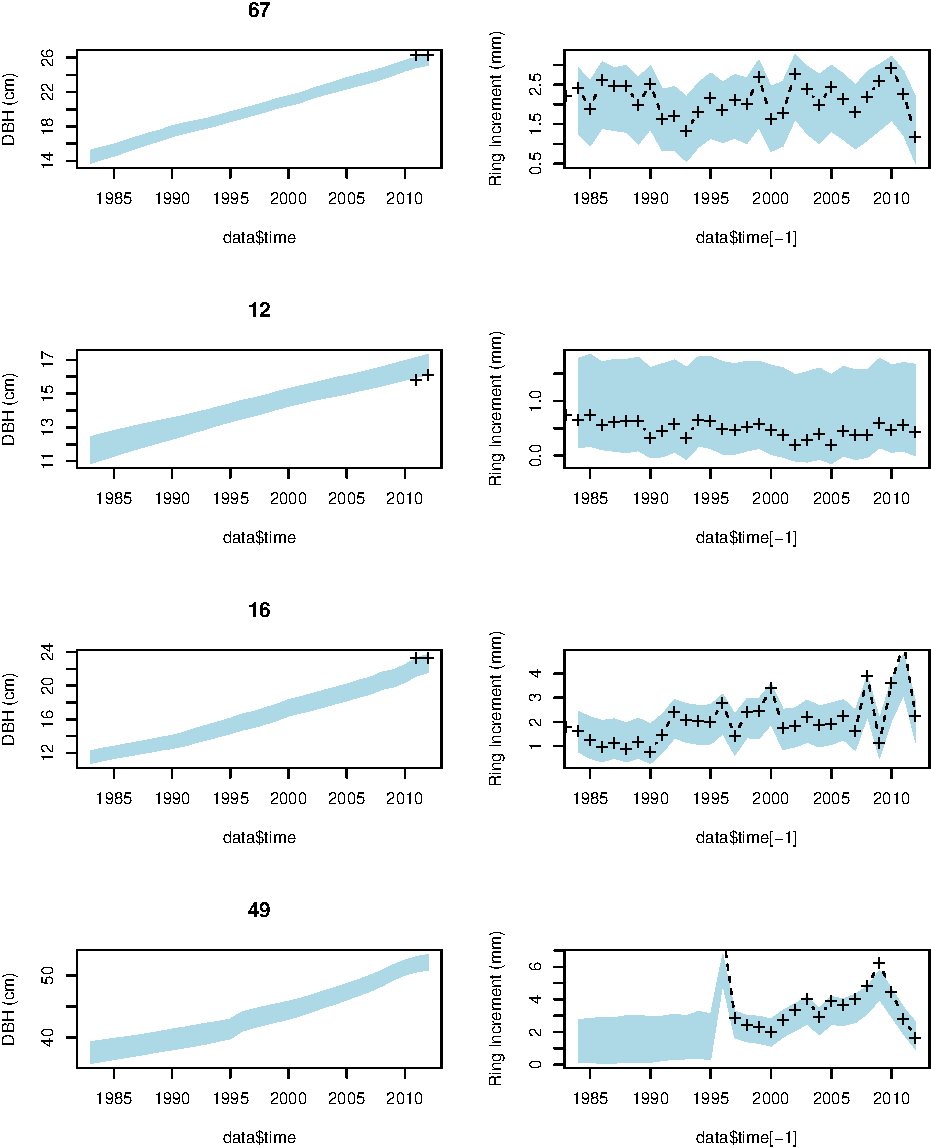
\includegraphics{Exercise_02_Logistic_files/figure-latex/unnamed-chunk-4-1.pdf}

This plot of the normal distribution and the effects of varying the
parameters in the normal are both probably familiar to you already --
changing the mean changes where the distribution is centered while
changing the standard deviation changes the spread of the distribution.
Next try looking at the CDF of the normal:

\begin{Shaded}
\begin{Highlighting}[]
\KeywordTok{plot}\NormalTok{(x,}\KeywordTok{pnorm}\NormalTok{(x,}\DecValTok{0}\NormalTok{,}\DecValTok{1}\NormalTok{),}\DataTypeTok{type=}\StringTok{'l'}\NormalTok{)}
\KeywordTok{abline}\NormalTok{(}\DataTypeTok{v=}\DecValTok{0}\NormalTok{)}
\KeywordTok{lines}\NormalTok{(x,}\KeywordTok{pnorm}\NormalTok{(x,}\DecValTok{2}\NormalTok{,}\DecValTok{1}\NormalTok{),}\DataTypeTok{col=}\DecValTok{2}\NormalTok{)}
\KeywordTok{abline}\NormalTok{(}\DataTypeTok{v=}\DecValTok{2}\NormalTok{,}\DataTypeTok{col=}\DecValTok{2}\NormalTok{)}
\KeywordTok{lines}\NormalTok{(x,}\KeywordTok{pnorm}\NormalTok{(x,}\OperatorTok{-}\DecValTok{1}\NormalTok{,}\DecValTok{2}\NormalTok{),}\DataTypeTok{col=}\DecValTok{3}\NormalTok{)}
\KeywordTok{abline}\NormalTok{(}\DataTypeTok{v=}\OperatorTok{-}\DecValTok{1}\NormalTok{,}\DataTypeTok{col=}\DecValTok{3}\NormalTok{)}
\end{Highlighting}
\end{Shaded}

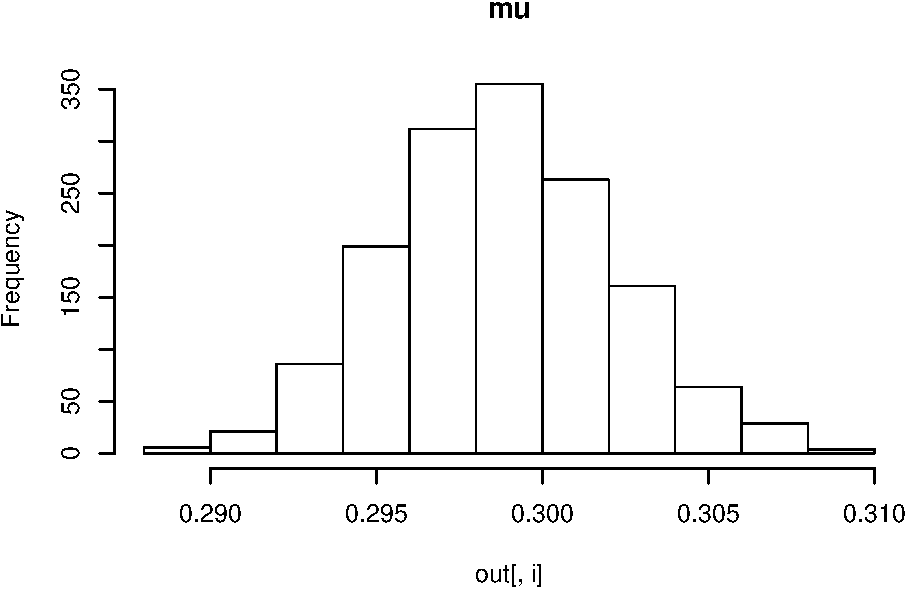
\includegraphics{Exercise_02_Logistic_files/figure-latex/unnamed-chunk-5-1.pdf}

Next let's look at the function qnorm. Since the input to this function
is a quantile, the x-values for the plot are restricted to the range
{[}0,1{]}.

\begin{Shaded}
\begin{Highlighting}[]
\NormalTok{p =}\StringTok{ }\KeywordTok{seq}\NormalTok{(}\DecValTok{0}\NormalTok{,}\DecValTok{1}\NormalTok{,}\DataTypeTok{by=}\FloatTok{0.01}\NormalTok{)}
\KeywordTok{plot}\NormalTok{(p,}\KeywordTok{qnorm}\NormalTok{(p,}\DecValTok{0}\NormalTok{,}\DecValTok{1}\NormalTok{),}\DataTypeTok{type=}\StringTok{'l'}\NormalTok{,}\DataTypeTok{ylim=}\KeywordTok{range}\NormalTok{(x))    }\CommentTok{# ylim sets the y-axis range}
\CommentTok{# range returns the min/max as a 2-element vector}
\KeywordTok{abline}\NormalTok{(}\DataTypeTok{h=}\DecValTok{0}\NormalTok{)                     }\CommentTok{# “h” for “horizontal”}
\KeywordTok{lines}\NormalTok{(p,}\KeywordTok{qnorm}\NormalTok{(p,}\DecValTok{2}\NormalTok{,}\DecValTok{1}\NormalTok{),}\DataTypeTok{col=}\DecValTok{2}\NormalTok{)}
\KeywordTok{abline}\NormalTok{(}\DataTypeTok{h=}\DecValTok{2}\NormalTok{,}\DataTypeTok{col=}\DecValTok{2}\NormalTok{)}
\KeywordTok{lines}\NormalTok{(p,}\KeywordTok{qnorm}\NormalTok{(p,}\OperatorTok{-}\DecValTok{1}\NormalTok{,}\DecValTok{2}\NormalTok{),}\DataTypeTok{col=}\DecValTok{3}\NormalTok{)}
\KeywordTok{abline}\NormalTok{(}\DataTypeTok{h=}\OperatorTok{-}\DecValTok{1}\NormalTok{,}\DataTypeTok{col=}\DecValTok{3}\NormalTok{)}
\end{Highlighting}
\end{Shaded}

\includegraphics{Exercise_02_Logistic_files/figure-latex/unnamed-chunk-6-1.pdf}

As you can see, the quantile function is the inverse of the CDF. This
function can be used to find the median of the distribution (p = 0.5) or
to estimate confidence intervals at any level desired.

\begin{Shaded}
\begin{Highlighting}[]
\KeywordTok{qnorm}\NormalTok{(}\KeywordTok{c}\NormalTok{(}\FloatTok{0.025}\NormalTok{,}\FloatTok{0.975}\NormalTok{),}\DecValTok{0}\NormalTok{,}\DecValTok{1}\NormalTok{)           }\CommentTok{# what width CI is specified by these values?}
\end{Highlighting}
\end{Shaded}

\begin{verbatim}
## [1] -1.959964  1.959964
\end{verbatim}

\begin{Shaded}
\begin{Highlighting}[]
\KeywordTok{plot}\NormalTok{(p,}\KeywordTok{qnorm}\NormalTok{(p,}\DecValTok{0}\NormalTok{,}\DecValTok{1}\NormalTok{),}\DataTypeTok{type=}\StringTok{'l'}\NormalTok{,}\DataTypeTok{ylim=}\KeywordTok{range}\NormalTok{(x))}
\KeywordTok{abline}\NormalTok{(}\DataTypeTok{v=}\KeywordTok{c}\NormalTok{(}\FloatTok{0.025}\NormalTok{,}\FloatTok{0.975}\NormalTok{),}\DataTypeTok{lty=}\DecValTok{2}\NormalTok{)  }\CommentTok{# add vertical lines at the CI}
\KeywordTok{abline}\NormalTok{(}\DataTypeTok{h=}\KeywordTok{qnorm}\NormalTok{(}\KeywordTok{c}\NormalTok{(}\FloatTok{0.025}\NormalTok{,}\FloatTok{0.975}\NormalTok{)),}\DataTypeTok{lty=}\DecValTok{2}\NormalTok{)   }\CommentTok{#add horizontal lines at the threshold vals}
\end{Highlighting}
\end{Shaded}

\includegraphics{Exercise_02_Logistic_files/figure-latex/unnamed-chunk-7-1.pdf}

\begin{Shaded}
\begin{Highlighting}[]
\KeywordTok{plot}\NormalTok{(x,}\KeywordTok{dnorm}\NormalTok{(x,}\DecValTok{0}\NormalTok{,}\DecValTok{1}\NormalTok{),}\DataTypeTok{type=}\StringTok{'l'}\NormalTok{)       }\CommentTok{# plot the corresponding pdf}
\KeywordTok{abline}\NormalTok{(}\DataTypeTok{v=}\KeywordTok{qnorm}\NormalTok{(}\KeywordTok{c}\NormalTok{(}\FloatTok{0.025}\NormalTok{,}\FloatTok{0.975}\NormalTok{)),}\DataTypeTok{lty=}\DecValTok{2}\NormalTok{)}
\end{Highlighting}
\end{Shaded}

\includegraphics{Exercise_02_Logistic_files/figure-latex/unnamed-chunk-7-2.pdf}

Finally, let's investigate the rnorm function for generating random
numbers that have a normal distribution. Here we generate histograms
that have a progressively larger sample size and compare that to the
actual density of the standard normal.

\begin{Shaded}
\begin{Highlighting}[]
\NormalTok{n =}\StringTok{ }\KeywordTok{c}\NormalTok{(}\DecValTok{10}\NormalTok{,}\DecValTok{100}\NormalTok{,}\DecValTok{1000}\NormalTok{,}\DecValTok{10000}\NormalTok{)    }\CommentTok{# sequence of sample sizes}
\ControlFlowTok{for}\NormalTok{(i }\ControlFlowTok{in} \DecValTok{1}\OperatorTok{:}\DecValTok{4}\NormalTok{)\{          }\CommentTok{# loop over these sample sizes}
  \KeywordTok{hist}\NormalTok{(}\KeywordTok{rnorm}\NormalTok{(n[i]),}\DataTypeTok{main=}\NormalTok{n[i],}\DataTypeTok{probability=}\OtherTok{TRUE}\NormalTok{,}\DataTypeTok{breaks=}\DecValTok{40}\NormalTok{)  }
                \CommentTok{#here breaks defines number of bins in the histogram}
  \KeywordTok{lines}\NormalTok{(x,}\KeywordTok{dnorm}\NormalTok{(x),}\DataTypeTok{col=}\DecValTok{2}\NormalTok{)}
\NormalTok{\}}
\end{Highlighting}
\end{Shaded}

\includegraphics{Exercise_02_Logistic_files/figure-latex/unnamed-chunk-8-1.pdf}
\includegraphics{Exercise_02_Logistic_files/figure-latex/unnamed-chunk-8-2.pdf}
\includegraphics{Exercise_02_Logistic_files/figure-latex/unnamed-chunk-8-3.pdf}
\includegraphics{Exercise_02_Logistic_files/figure-latex/unnamed-chunk-8-4.pdf}

One other technical note: like any function in R that generates random
output, this example will give different results every time you run it.

This example demonstrates that as the number of random draws from a
probability distribution increases, the histogram of those draws
provides a better and better approximation of the density itself. We
will make use of this fact extensively this semester because -- as odd
as this may sound now -- there are many distributions that are easier to
randomly sample from than solve for analytically.

\subsubsection{Problems}\label{problems-1}

\begin{enumerate}
\def\labelenumi{\arabic{enumi}.}
\setcounter{enumi}{1}
\tightlist
\item
  Choose another probability distribution and generate graphs of the
  probability density function, the cumulative distribution function,
  the quantile function, and a histogram of samples from that
  distribution.
\end{enumerate}

\subsection{Monte Carlo Simulation}\label{monte-carlo-simulation}

Most of the figures from the logistic growth example in Chapter 2
included plots of the median trajectory and 95\% interval estimates.
These summary statistics are a reflection of the fact that the
underlying model prediction was a timeseries of probability
distributions, rather than a single trajectory. So how do we project a
probability distribution through time?

In Chapter 11 we will explore a variety of analytical and numerical
approachs to propagating uncertainty, and the trade-offs among them, in
much greater detail. Today I wanted to introduce a particularly common
and general numerical approach, \textbf{Monte Carlo} simulation. A Monte
Carlo method is any algorithm that relys on randomization to approximate
a computation. These approaches and other will be discussed in more
detail later (e.g.~Chapters 5, 11, 13, \& 14).

The previous example of approximating the Normal distribution with a
histogram of samples from the Normal distribution is a simple
illustration of this approach. What makes this approach powerful is that
we can transform the samples from a distribution through whatever
function we would like and the resulting set of samples is the correct
histogram for that transformation. This is important because, by
contrast, we \textbf{cannot} transform the summary statistics, such as
the mean of the probability distribution, through an arbitrary function
because of \textbf{Jensen's Inequality}.

To illustrate this point, consider the function x\^{}2 and a standard
Normal distribution (mean = 0, sd = 1). Now if we ignore Jensen's
Inequality and tranform the mean and 95\% CI we'd end up with a
probability distribution that has a mean of 0\^{}2 = 0, a lower
confidence interval of -1.96\^{}2 = 3.84 and an upper confidence
interval of 1.96\^{}2 = 3.84. Clearly this can't be correct, since the
upper and lower CI are identical and the lower CI is higher than the
mean. By contrast, if we do this transformation numerically

\begin{Shaded}
\begin{Highlighting}[]
\NormalTok{x =}\StringTok{ }\KeywordTok{rnorm}\NormalTok{(}\DecValTok{10000}\NormalTok{,}\DecValTok{0}\NormalTok{,}\DecValTok{1}\NormalTok{)}
\NormalTok{y =}\StringTok{ }\NormalTok{x}\OperatorTok{^}\DecValTok{2}

\KeywordTok{hist}\NormalTok{(x,}\DataTypeTok{main=}\StringTok{"Original distribution"}\NormalTok{,}\DataTypeTok{breaks=}\DecValTok{40}\NormalTok{)}
\KeywordTok{abline}\NormalTok{(}\DataTypeTok{v=}\KeywordTok{quantile}\NormalTok{(x,}\KeywordTok{c}\NormalTok{(}\FloatTok{0.025}\NormalTok{,}\FloatTok{0.5}\NormalTok{,}\FloatTok{0.975}\NormalTok{)),}\DataTypeTok{lty=}\KeywordTok{c}\NormalTok{(}\DecValTok{2}\NormalTok{,}\DecValTok{1}\NormalTok{,}\DecValTok{2}\NormalTok{),}\DataTypeTok{lwd=}\DecValTok{3}\NormalTok{,}\DataTypeTok{col=}\StringTok{"orange"}\NormalTok{)}
\KeywordTok{abline}\NormalTok{(}\DataTypeTok{v=}\KeywordTok{mean}\NormalTok{(x),}\DataTypeTok{col=}\StringTok{"red"}\NormalTok{,}\DataTypeTok{lwd=}\DecValTok{3}\NormalTok{,}\DataTypeTok{lty=}\DecValTok{3}\NormalTok{)}
\end{Highlighting}
\end{Shaded}

\includegraphics{Exercise_02_Logistic_files/figure-latex/unnamed-chunk-9-1.pdf}

\begin{Shaded}
\begin{Highlighting}[]
\KeywordTok{hist}\NormalTok{(y,}\DataTypeTok{main=}\StringTok{"Transformed distribution"}\NormalTok{,}\DataTypeTok{breaks=}\DecValTok{40}\NormalTok{)}
\KeywordTok{abline}\NormalTok{(}\DataTypeTok{v=}\KeywordTok{quantile}\NormalTok{(y,}\KeywordTok{c}\NormalTok{(}\FloatTok{0.025}\NormalTok{,}\FloatTok{0.5}\NormalTok{,}\FloatTok{0.975}\NormalTok{)),}\DataTypeTok{lty=}\KeywordTok{c}\NormalTok{(}\DecValTok{2}\NormalTok{,}\DecValTok{1}\NormalTok{,}\DecValTok{2}\NormalTok{),}\DataTypeTok{lwd=}\DecValTok{3}\NormalTok{,}\DataTypeTok{col=}\StringTok{"orange"}\NormalTok{)}
\KeywordTok{abline}\NormalTok{(}\DataTypeTok{v=}\KeywordTok{mean}\NormalTok{(y),}\DataTypeTok{col=}\StringTok{"red"}\NormalTok{,}\DataTypeTok{lwd=}\DecValTok{3}\NormalTok{,}\DataTypeTok{lty=}\DecValTok{3}\NormalTok{)}
\end{Highlighting}
\end{Shaded}

\includegraphics{Exercise_02_Logistic_files/figure-latex/unnamed-chunk-9-2.pdf}

The Monte Carlo estimate is that the mean is 1.0079112, the median is
0.4523527, and the 95\% CI is 7.7469496\times 10\^{}\{-4\}, 4.9774902.

It turns out that this specific transformation (x\^{}2 of a standard
Normal), has a well known analytical solution -- a Chi-squared
distribution with one degee of freedom, so in this case we can compare
the numerical approximation with the exact solution. This Chi-squared
has a mean of 1, a median of 0.4549364 and a 95\% CI of
9.8206912\times 10\^{}\{-4\}, 5.0238862.

\subsubsection{Problems}\label{problems-2}

\begin{enumerate}
\def\labelenumi{\arabic{enumi}.}
\setcounter{enumi}{2}
\tightlist
\item
  Numerically transform a lognormal(meanlog=0,sdlog=0.5) through sin(x)
  using Monte Carlo simulation. Include histograms of the original and
  transformed distributions. Report the mean, median, and 95\% CI for
  both distributions and indicate these values on the histograms.
\end{enumerate}

\subsection{Parameter error}\label{parameter-error}

We next want to use the Monte Carlo approach to account for parameter
uncertainty in the logistic growth model

To begin, we need to specify the uncertainty in the model parameters and
the size of the simulation

\begin{Shaded}
\begin{Highlighting}[]
\NormalTok{r.sd =}\StringTok{ }\FloatTok{0.2}\NormalTok{     ## standard deviation on r}
\NormalTok{K.sd =}\StringTok{ }\FloatTok{1.0}\NormalTok{     ## standard deviation on K}
\NormalTok{NE =}\StringTok{ }\DecValTok{1000}\NormalTok{      ## Ensemble size}
\end{Highlighting}
\end{Shaded}

Next, we need to run the Monte Carlo simulation for the logistic. In
this case we'll be running the logistic growth model 1000 times, each
time with slightly different parameters. We'll then store all 1000
trajectories in a matrix. In effect, we'll be estimating our probability
distributions and all of our summary statistics from a sample of
time-series, rather than a sample of points as we did in the previous
example.

\begin{Shaded}
\begin{Highlighting}[]
\NormalTok{n =}\StringTok{ }\KeywordTok{matrix}\NormalTok{(n0,NE,NT)   }\CommentTok{# storage for all simulations}
\NormalTok{rE =}\StringTok{ }\KeywordTok{rnorm}\NormalTok{(NE,r,r.sd)  }\CommentTok{# sample of r}
\NormalTok{KE =}\StringTok{ }\KeywordTok{rnorm}\NormalTok{(NE,K,K.sd)  }\CommentTok{# sample of K}
\ControlFlowTok{for}\NormalTok{(i }\ControlFlowTok{in} \DecValTok{1}\OperatorTok{:}\NormalTok{NE)\{        }\CommentTok{# loop over samples}
  \ControlFlowTok{for}\NormalTok{(t }\ControlFlowTok{in} \DecValTok{2}\OperatorTok{:}\NormalTok{NT)\{      }\CommentTok{# for each sample, simulate throught time}
\NormalTok{    n[i,t] =}\StringTok{ }\NormalTok{n[i,t}\OperatorTok{-}\DecValTok{1}\NormalTok{] }\OperatorTok{+}\StringTok{ }\NormalTok{rE[i]}\OperatorTok{*}\NormalTok{n[i,t}\OperatorTok{-}\DecValTok{1}\NormalTok{]}\OperatorTok{*}\NormalTok{(}\DecValTok{1}\OperatorTok{-}\NormalTok{n[i,t}\OperatorTok{-}\DecValTok{1}\NormalTok{]}\OperatorTok{/}\NormalTok{KE[i])}
\NormalTok{  \}}
\NormalTok{\}}
\end{Highlighting}
\end{Shaded}

Next we'll use \emph{apply} to calculate the median and CI for each time
point.

\begin{Shaded}
\begin{Highlighting}[]
\NormalTok{n.stats =}\StringTok{ }\KeywordTok{apply}\NormalTok{(n,}\DecValTok{2}\NormalTok{,quantile,}\KeywordTok{c}\NormalTok{(}\FloatTok{0.025}\NormalTok{,}\FloatTok{0.5}\NormalTok{,}\FloatTok{0.975}\NormalTok{))}
\end{Highlighting}
\end{Shaded}

\subsubsection{Problems}\label{problems-3}

\begin{enumerate}
\def\labelenumi{\arabic{enumi}.}
\setcounter{enumi}{3}
\item
  Plot histograms of the samples of r and K used for the simulation.
\item
  Plot a sample of 10 different trajectories (through time) from your
  ensemble (on one graph).
\item
  Plot a histogram of your population forecast at time = 15.
\item
  Plot the median trajectory through time. Use
  \texttt{ecoforecastR::ciEnvelope} to add a 95\% CI (i.e.~2.5\% to
  97.5\%) to the plot. This function need to take time-series for both
  the upper (yhi) and lower (ylo) intervals.
\end{enumerate}

\subsection{Extra Credit: Initial
conditions}\label{extra-credit-initial-conditions}

The approach for simulating uncertainty in the initial conditions is
very similar to the approach used for the parameter uncertainty. As in
Chapter 2, we'll assume that the initial condition is distributed as a
lognormal to ensure that we never draw negative values. For this example
we'll assume a standard deviation of 0.6 and an intrinsic growth rate of
0.3

\begin{Shaded}
\begin{Highlighting}[]
\NormalTok{r =}\StringTok{ }\FloatTok{0.3}
\NormalTok{n0.sd =}\StringTok{ }\FloatTok{0.6}
\NormalTok{n0s =}\StringTok{ }\KeywordTok{rlnorm}\NormalTok{(NE,}\KeywordTok{log}\NormalTok{(n0),n0.sd)}
\NormalTok{n =}\StringTok{ }\KeywordTok{matrix}\NormalTok{(n0s,NE,NT)}
\ControlFlowTok{for}\NormalTok{(i }\ControlFlowTok{in} \DecValTok{1}\OperatorTok{:}\NormalTok{NE)\{}
  \ControlFlowTok{for}\NormalTok{(t }\ControlFlowTok{in} \DecValTok{2}\OperatorTok{:}\NormalTok{NT)\{}
\NormalTok{    n[i,t] =}\StringTok{ }\NormalTok{n[i,t}\OperatorTok{-}\DecValTok{1}\NormalTok{] }\OperatorTok{+}\StringTok{ }\NormalTok{r}\OperatorTok{*}\NormalTok{n[i,t}\OperatorTok{-}\DecValTok{1}\NormalTok{]}\OperatorTok{*}\NormalTok{(}\DecValTok{1}\OperatorTok{-}\NormalTok{n[i,t}\OperatorTok{-}\DecValTok{1}\NormalTok{]}\OperatorTok{/}\NormalTok{K)}
\NormalTok{  \}}
\NormalTok{\}}
\end{Highlighting}
\end{Shaded}

\subsubsection{Problems}\label{problems-4}

\begin{enumerate}
\def\labelenumi{\arabic{enumi}.}
\setcounter{enumi}{7}
\item
  Plot the median \& 95\% interval.
\item
  Repeat with r equal to 1.95, 2.05, and 2.8
\end{enumerate}


\end{document}
